% Template for Cogsci submission with R Markdown

% Stuff changed from original Markdown PLOS Template
\documentclass[10pt, letterpaper]{article}

\usepackage{cogsci}
\usepackage{pslatex}
\usepackage{float}

% amsmath package, useful for mathematical formulas
\usepackage{amsmath}

% amssymb package, useful for mathematical symbols
\usepackage{amssymb}

% hyperref package, useful for hyperlinks
\usepackage{hyperref}

% graphicx package, useful for including eps and pdf graphics
% include graphics with the command \includegraphics
\usepackage{graphicx}

% Sweave(-like)
\usepackage{fancyvrb}
\DefineVerbatimEnvironment{Sinput}{Verbatim}{fontshape=sl}
\DefineVerbatimEnvironment{Soutput}{Verbatim}{}
\DefineVerbatimEnvironment{Scode}{Verbatim}{fontshape=sl}
\newenvironment{Schunk}{}{}
\DefineVerbatimEnvironment{Code}{Verbatim}{}
\DefineVerbatimEnvironment{CodeInput}{Verbatim}{fontshape=sl}
\DefineVerbatimEnvironment{CodeOutput}{Verbatim}{}
\newenvironment{CodeChunk}{}{}

% cite package, to clean up citations in the main text. Do not remove.
\usepackage{cite}

\usepackage{color}

% Use doublespacing - comment out for single spacing
%\usepackage{setspace}
%\doublespacing


% % Text layout
% \topmargin 0.0cm
% \oddsidemargin 0.5cm
% \evensidemargin 0.5cm
% \textwidth 16cm
% \textheight 21cm

\title{Reaction times in processing scalar implicatures}


\author{{\large \bf Rose M. Schneider} \\ \texttt{rschneid@stanford.edu} \\ Department of Psychology \\ Stanford University \And {\large \bf Michael C. Frank} \\ \texttt{mcfrank@stanford.edu} \\ Department of Psychology \\ Stanford University}

\begin{document}

\maketitle

\begin{abstract}
Children's trouble with scalar implicatures -- inferences from a weaker
lexicalized description that a stronger alternative is true -- is a
puzzle in pragmatic development. Previous research indicates that
children's failures in processing scalar implicatures may be rooted in
an unestablished quantifier scale, with children who struggle with the
quantifier ``some'' being unable to contrast different quantifiers to
make the implicature. However, the source of this failure is unclear.
Here, we explore reaction time as a measure of processing for scalar
implicatures (and reasoning about salient alternatives, such as
``none''). In our analyses, we explore overall performance and reaction
time patterns across development, finding that increased reaction times
and accuracy for the quantifiers ``some'' and ``none.'' Motivated by
these findings, we use a Drift Diffusion Model to explore the
relationship between accuracy and reaction time in processing both
scalar implicatures, and the quantifiers ``some'' and ``none'' more
broadly. Overall, we find evidence that while children's performance in
scalar implicature tasks is hindered by absent quantifier knowledge,
their success also requires additional processing when reasoning about
that quantifier scale.

\textbf{Keywords:}
Pragmatics; development; language.
\end{abstract}

\section{Introduction}\label{introduction}

In listening to language, we are presented with a large amount of
information to process in a very short period of time. For the most
part, we're successful communicators, and can integrate linguistic
information quickly and efficiently. How do we develop this ability,
particularly in challenging pragmatic contexts where meaning is not
stated, but implied? When we do make errors, where does the language
comprehension process break down? We know that early in development,
children often stumble in comprehending language. A particularly salient
and well-researched example of this pragmatic development is
preschoolers' failures in making scalar implicatures. What can
children's difficulties in this case reveal about breakdowns in language
comprehension more broadly?

In comprehending language, as listeners we have available to us not only
a speaker's verbalized statement, but also the knowledge of what the
speaker \emph{could} have said. In fact, listeners frequently go beyond
the literal sense of utterances to infer a speaker's intended meaning.
In the case of \emph{pragmatic implicatures} (Grice, 1975), a weaker
literal description can imply that a stronger alternative is true. Thus,
an adult listener would strongly infer from the statement ``I enjoyed
\emph{some} of my winter break'' that some (but not \emph{all}) of my
break was pleasant. This \emph{scalar implicature} (SI) relies heavily
on a knowledge of the relevant lexical alternatives in the quantifier
scale \(<\)none, some, all\(>\), as a listener must be able to contrast
these alternatives in computing the implicature. While scalar
implicatures are easily comprehended by adults, they pose a pragmatic
challenge to children until fairly late in development (Horowitz \&
Frank, 2015; Katsos \& Bishop, 2011; Papafragou \& Musolino, 2003). What
is the source of children's difficulties with scalar implicatures?

In contrast to adults' spontaneous processing of such pragmatic
implicatures, children display marked and striking failures in such
tasks. For example, when judging a scene in which three of three horses
have jumped over a fence, preschoolers are likely to endorse the
statement ``\emph{All} of the horses jumped over the fence'' as
felicitous, rather than the appropriate statement ``\emph{Some} of the
horses jumped over the fence'' (Papafragou \& Musolino, 2003). Across
different studies, however, children exhibit varying performance,
depending on the paradigm, syntactic construction of the implicature
prompts, access to visual and lexical alternatives, and age (Guasti et
al., 2005; Horowitz \& Frank, 2015; Noveck, 2001; Papafragou \&
Musolino, 2003; Papafragou \& Tantalou, 2004). Making inferences from
these various datasets about the source of children's failures in making
scalar implicatures is made difficult by various measures and tasks
uses.

In an attempt to reconcile these various accounts, Horowitz and Frank
(2015) designed a simple referent selection paradigm that could be used
across a broad age range (3--5 years) to explore lexicalized (scalar)
implicatures. In this task, children saw three book covers, each
featuring four familiar objects (Figure \ref{fig:image}), and the
experimenter described a book using either a scalar (quantifier)
description (e.g., ``On the cover of my book, \emph{none/some/all} of
the pictures are cats.''). Children's responses were scored as correct
if they selected the book consistent with the quantifier description.

\begin{CodeChunk}
\begin{figure}[b]

{\centering 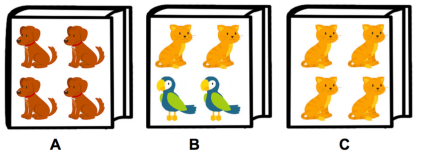
\includegraphics{figs/image-1} 

}

\caption[Example trial stimuli used in Horowitz and Frank (2015)]{Example trial stimuli used in Horowitz and Frank (2015).}\label{fig:image}
\end{figure}
\end{CodeChunk}

Using this paradigm, Horowitz and Frank found children struggled with
the quantifiers ``some'' and ``none'' in relation to ``all'', although
performance increased across development. Intriguingly, they found that
performance between these two quantifiers was strongly bimodal and
correlated: Children who failed on trials with the quantifier ``some''
similarly struggled with ``none,'' and vice versa.

Children's failures in computing scalar implicatures, and their related
performance processing the quantifiers ``some'' and ``none'' presented
two hypotheses for sources of developmental difficulty in this task,
namely, lack of quantifier knowledge and developing inhibitory control
(Horowitz, Schneider, \& Frank, In prep.). Making a scalar implicature
requires familiarity with and ability to contrast alternatives on the
quantifier scale \(<\)\emph{none -- some -- all}\(>\); if children's
quantifier knowledge is absent or unestablished, it might lead to
failures in making an implicature. Alternatively, children may have
complete quantifier knowledge, but are unable to inhibit an impulse to
choose a more salient alternative.

Horowitz et al. explored these two hypotheses in an individual
differences task, running their scalar implicature (Horowitz \& Frank,
2015) task in conjunction with a quantifier-knowledge (Barner, Chow, \&
Yang, 2009) and inhibitory control (Zelazo, 2006) tasks. Overall, they
found that children's scalar implicature performance was strongly
correlated with quantifier knowledge, even when controlling for age.
While inhibitory control was strongly correlated with age, it was not
related to children's performance on the SI task (Horowitz et al., In
prep.).

While the ability to compute a scalar implicature seems to be closely
related to knowledge of the complete quantifier scale (rather than pure
inhibitory control), it is likely that children's failures have several
underlying causes. In particular, an unexplored (and more nuanced)
measure of inhibitory control is the response latency associated with
making an implicature. Here, we explore children's response times in
Horowitz and Frank's (2015) task as a measure of inhibitory control. To
obtain accurate reaction times, we adapted the task for an iPad, and
expanded the sample size.

In our analyses, we explore overall accuracy and patterns of
performance, as in (Horowitz \& Frank, 2015; Horowitz et al., In prep.),
and find that children not only struggle in making a scalar implicature,
but also grapple with the quantifier ``none'' until fairly late in
development. In examining reaction time patterns across all quantifier
types, we find a speed-accuracy tradeoff associated with these two
quantifiers, even later in development. Finally, we use a Drift
Diffusion Model to our data, and find that longer response latencies are
predictive of success in computing a scalar implicature, and
understanding the quantifier ``none.'' Overall, our findings indicate
that while quantifier knowledge is a key factor in successfully
computing scalar implicatures, using this information to successfully
compute a scalar implicature is particularly difficult, and requires
additional processing.

\section{General Methods}\label{general-methods}

In this study, we adapted a Scalar Implicature paradigm developed by
Horowitz and Frank (2015) for the iPad. In addition to capturing
detailed reaction time data, this version included more trials, and
standardized prosody across all trials, in addition to a completely
randomized design.
\footnote{All of our data, processing, and analysis code can be viewed in the version control repository for this paper at: https://github.com/rosemschneider/SI\_tablet.}

\subsubsection{Participants}\label{participants}

125 out of a planned sample of 120 was recruited from Bing Nursery
School at Stanford University and the Children's Discovery Museum in San
Jose. Participants ranged in age from 3--6.5 years: 19 3--3.5-year-olds
(M = 3.3, median = 3.32, SD = 0.13); 31 3.5--4-year-olds (M = 3.79,
median = 3.75, SD = 0.15); 23 4--4.5-year-olds (M = 4.28, median = 4.28,
SD = 0.15); 28 4.5--5-year-olds (M = 4.75, median = 4.74, SD = 0.15);
and 24 5--6.5-year-olds (M = 5.55, median = 5.56, SD = 0.36). Two
additional children were run, but were excluded as out of the age range.
Based on (Horowitz \& Frank, 2015; Horowitz et al., In prep.), the
initially planned sample size was 96 children from 3--5 years. After
collecting data from 57 participants, however, we observed significantly
lower performance on critical trials across all age groups, indicating
that the iPad adaptation of the scalar implicature task was slightly
more challenging for all children. With this extended developmental
trajectory in mind, we decided to include an older age group of
twenty-four 5--6.5-year-olds.

\subsubsection{Stimuli}\label{stimuli}

The general format of the task was identical to (Horowitz \& Frank,
2015), with the exception of added items for additional trials. The
study was programmed in HTML, CSS, and JavaScript, and displayed to
children on full-sized iPad. Each trial displayed three book covers,
each containing a set of four familiar objects (Figure \ref{fig:image}).
Each trial allowed 2.5s for children to visually inspect the three book
covers, before the experiment played the trial prompt (e.g., ``On the
cover of my book, \emph{none} of the pictures are cats.''). Each trial
was completely randomized, with the exception that similar items were
displayed together (e.g., food, clothing). Each session involved 30
trials, with 10 trials per quantifier-type (``all'', ``some'', and
``none''). In our randomization, quantifier triad order, items (within
category), target item, and quantifier, were randomized for all
participants.

\subsubsection{Procedure}\label{procedure}

Sessions took place individually in a small testing room away from
either the museum or the nursery school. Each session began with the
child playing the ``dot game,'' which required them to press dots on the
iPad screen as fast as they could. This game was included to familiarize
children with the iPad.

After children finished the dot game, the experimenter introduced them
to ``Hannah,'' a cartoon character who wanted to play a guessing game
with her books. The experimenter explained that Hannah would show the
child three books, and would give the child \emph{one} hint about which
book she was thinking of. The experimenter emphasized that Hannah would
only give one hint, so they had to listen carefully. Children then saw a
practice trial with three books featuring a refrigerator, a TV, and a
couch. After 2.5s, a female voice said ``On the cover of my book there's
a TV.'' Once children correctly made their selection, a green box
appeared around the selection. Children moved trials along at their own
pace by pressing a green button that appeared after they had made their
selection.

Reaction times were measured from the onset of the target word. Each
audio clip used the same three frames (e.g., ``On the cover of my book,
\emph{some} of the pictures\ldots{}'') so that prodosdy was emphasized
equally across all trials. Across all trials, the average length of each
audio clip (including target item phrase, e.g., ``\ldots{}are cats'')
was approximately 6s. In all, there were 270 different target items and
audio clips.

Children could only make one selection. If a child was not paying
attention, or if she did not hear Hannah's prompt, the experimenter
repeated it, matching the original prosody.

\section{Results}\label{results}

In analyzing the results, we excluded any trials in which reaction time
exceeded thirty seconds, which indicated that the child had missed the
prompt, or was not paying attention. After this initial cut, we excluded
responses outside three standard deviations of the log of the reaction
time mean. This cleaning process resulted in a data loss of 75 trials
(2.08\%).

\subsection{Accuracy}\label{accuracy}

\begin{CodeChunk}
\begin{figure}[h]
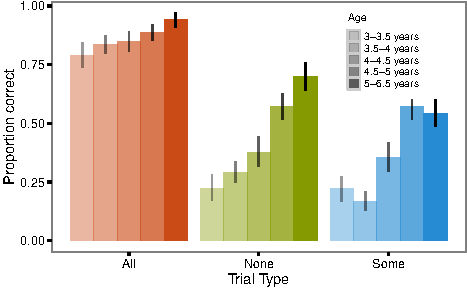
\includegraphics{figs/overall_acc-1} \caption[Children's overall accuracy for each quantifier type]{Children's overall accuracy for each quantifier type. Bars show mean performance for each age group. Error bars are 95 percent confidence intervals computed by non-parametric bootstrap.}\label{fig:overall_acc}
\end{figure}
\end{CodeChunk}

In our first planned analysis, we explored children's overall patterns
of accuracy for each quantifier type. Figure \ref{fig:overall_acc} shows
children's performance for each quantifier type. For each age group, we
saw significantly lower accuracy for the quantifiers ``some'' and
``none'' in comparison to ``all'' in independent t-tests within each age
group (\(p\) \textless{} .01 for all tests). This replication of
previous results using this paradigm (Horowitz \& Frank, 2015; Horowitz
et al., In prep.) indicates that our iPad adaptation of this task is an
appropriate measure.

Because our adaptation relies strictly on verbal communication, however,
it may prove more difficult for children, resulting in lowered
performance across all age groups. We found that children lose some
communicative power when relying only on linguistic information in this
task. Children aged 3--5 years perform significantly lower on ``some''
(implicature) trials in this task in comparison with (Horowitz et al.,
In prep.) in independent t-tests (\(p\) \textless{} .05 for all tests).
We believe that the lower performance on this task is the result of a
more challenging experimental context, rather than developmental
pragmatic failures.

\subsubsection{Statistical modeling}\label{statistical-modeling}

In exploring children's signficantly lower performance on ``some'' and
``none'' trials, we ran a logistic mixed effects model predicting
correct response as an interaction of age and trial type, with random
effects of trial type and participant.
\footnote{Mixed effects model fit in R using the lme4 package. The model specifications were as follows: \texttt{correct ~ age * trial type + (trial type | subject id)}.}
We found that performance was significantly lower on ``some'' (\(\beta\)
= -8.14, \(p\) \textless{} .0001) and ``none'' trials (\(\beta\) =
-11.36, \(p\) \textless{} .0001). We also found a signficant interaction
between age and trial type on ``none'' trials(\(\beta\) = 1.89, \(p\)
\textless{} .0001), indicating that children's performance with this
difficult quantifier increased with age.

\subsubsection{Correlation between ``some'' and
``none''}\label{correlation-between-some-and-none}

\begin{CodeChunk}
\begin{figure}[h]
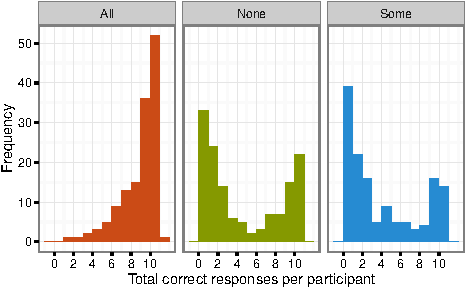
\includegraphics{figs/diptest-1} \caption[Frequency histogram of correct responses for each trial type, across all participants]{Frequency histogram of correct responses for each trial type, across all participants.}\label{fig:diptest}
\end{figure}
\end{CodeChunk}

In previous research, a strong correlation has been found on children's
performance with the quantifiers ``some'' and ``none'' (Horowitz \&
Frank, 2015; Horowitz et al., In prep.). Once again, we found correlated
performance between these two quantifiers (\(r\) = 0.47, \(p\)
\textless{} .001). In running Hartigan's diptest for bimodality on these
two quantifiers, we found significant bimodal distributions for ``some''
(\(D\) = 0.08, \(p\) \textless{} 0) and ``none'' trials (\(D\) = 0.11,
\(p\) \textless{} .00001). While we also found that Hartigan's diptest
indicated that performance in ``all'' trials was not signficantly
unimodal (\(D\) = 0.12, \(p\) \textless{} .00001), this is most likely
due to the large number of participants and trials in our study, as
performance on ``all'' trials (Figure \ref{fig:diptest}) shows strong
evidence of unimodality. These values indicate that while children's
accuracy is significantly worse on ``some'' and ``none'' trials, their
performance is consistent, and that they make their responses in
meaningful manner over the course of the study.

\subsection{Reaction time analyses}\label{reaction-time-analyses}

A previously-unexplored aspect of children's ability to compute scalar
implicatures is their reaction time on these kinds of pragmatic tasks.
Huang and Snedeker (2009) explored eye-movements as a measure of online
pragmatic processing; response latencies in behavioral implicature data,
however, remainly largely unknown. We hypothesized that children's
reaction times on this task may be a measure of the processing involved
in comprehending the quantifiers ``some'' and ``none.'' It is possible
that this more nuanced measure of inhibitory control may provide a clue
as to the nature of children's correlated struggles with these terms. In
recording reaction times, we began recording from the onset of the
target nouns, and measured in milliseconds. Here, we explore overall
trends in reaction times across this task, and the relationship between
response latencies and accuracy on this task.

\subsubsection{Developmental reaction time
distribution\\}\label{developmental-reaction-time-distribution}

Figure \ref{fig:rt_spread} shows the distribution of reaction times for
each quantifier, faceted by age group. Overall, we found that reaction
time was negatively correlated with age (\emph{r} = -0.25, \emph{p}
\textless{} .0001). In exploring the relationship between accuracy and
reaction time, we found preliminary evidence of a speed-accuracy
tradeoff across all trial types (Figure \ref{fig:density}) shows the
density of reaction times for correct and incorrect selections for each
quantifier type.

\begin{CodeChunk}
\begin{figure*}[t]

{\centering 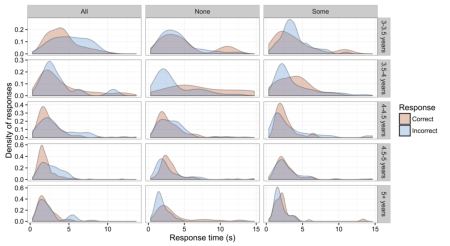
\includegraphics{figs/density-1} 

}

\caption[Density plots of reaction times for correct and incorrect responses on each trial type, split by age]{Density plots of reaction times for correct and incorrect responses on each trial type, split by age.}\label{fig:density}
\end{figure*}
\end{CodeChunk}

Figure \ref{fig:density} also shows evidence for increased response
latencies associated with the quantifiers ``some'' and ``none,''
especially early in development, reflecting the difficulty in processing
these terms. Overall, we found that children were largely consistent in
their performance across the course of the study in reaction time
correlations between ``all'' and ``some'' (\emph{r} = 0.76, \emph{p}
\textless{} .0001), ``all'' and ``none'' (\emph{r} = 0.76, \emph{p}
\textless{} .0001), and ``some'' and ``none'' trials (\emph{r} = `r
round(somenone\_corr\$estimate, 2), \emph{p} \textless{} .0001).

\subsubsection{Statistical modeling}\label{statistical-modeling-1}

We next turned to the relationship betwen age, reaction time, and
accuracy. Our initial hypothesis was that computing quantifiers is
pragmatically difficult, and doing so successfully may require
additional processing time. In exploring this, we ran a planned linear
mixed effects model predicting response time as an interaction of age,
trial number, and trial type with a random effect of trial type.
\footnote{Mixed effects model fit in R using the lme4 package. The model specifications were as follows: \texttt{log(reaction time) ~ scale(age) * log(trial number) + scale(age) * trial type + (trial type | subject id)}. We calculated \emph{p} values by treating the \emph{t} statistic as if it were a \emph{z} statistic [@barr2013].}
We found a main effect of trial number, with reaction times decreasing
over the course of the study ((\(\beta\) = -0.11, \(p\) \textless{}
.00001)), but found that reaction times significantly increased on
``none'' (\(\beta\) = 0.22, \(p\) \textless{} .00001), and ``some''
trials (\(\beta\) = 0.1, \(p\) \textless{} .00001). Interestingly, we
also found an interaction between age and trial type, such reaction time
on ``none'' and ``some'' trials increased with age (``None'': (\(\beta\)
= -0.01, \(p\) \textless{} .00001; ``Some'': (\(\beta\) = 0.14, \(p\)
\textless{} .004).

This interaction is particularly intriguing because in our previous
accuracy model, we found increased performance on these trial types.
While we find that older children are taking longer to respond to these
trial types, they are more likely to get them correct, even though
reaction time is negatively correlated with age. This seems to indicate
that succesfully comprehending these difficult scalar terms does require
additional processing time.

\subsection{Drift diffusion models}\label{drift-diffusion-models}

In our previous statistical models, we observed a speed-accuracy
tradeoff in older children's performance on ``some'' and ``none''
trials. This suggests that children may be taking more time to process
these particular quantifiers as they become more familiar with the
quantifier scale. A drift diffusion model (DDM) can provide a more
detailed view of the relationship between accuracy and reaction time in
behavioral tasks (Milosavljevic, Malmaud, Huth, Koch, \& Rangel, 2010).
\footnote{While DDMs are traditionally used to examine two-alternative forced-choice behavioral decisions, here we use the model to predict the relationship between reaction time and accuracy in making either a correct or incorrect decision in our task.}

\subsubsection{Parameter estimation}\label{parameter-estimation}

In DDM, a behavioral response (a correct or incorrect choice) is the
result of noisy data accumulation (operationalized by response time)
(Ratcliff \& Rouder, 1998). Responses have \emph{separation boundaries}
that are dependent on the amount of information needed to initate a
response, and \emph{drift rate} formalizes the rate of data accumulation
(Ratcliff \& Rouder, 1998). An additional parameter of DDM is
\emph{nondecision}, which is the amount of time between encoding the
stimuli, and initiating response. Finally, different responses may have
a \emph{bias}, or different starting point in the diffusion process,
dependent on the stimuli (Ratcliff \& Rouder, 1998).

In fitting a DDM to our data, we estimated parameters for each subject
across all three trial types (``all'', ``some'', and ``none'') using the
RWiener package. We then aggregated across subjects to obtain means and
confidence intervals for each age group.
\footnote{Here we should address reaction time exclusion, when we've made a decision about it.}
Figure \ref{fig:param_plot} shows the parameter estimates for each age
group, split by trial type.

\begin{CodeChunk}
\begin{figure*}[t]

{\centering 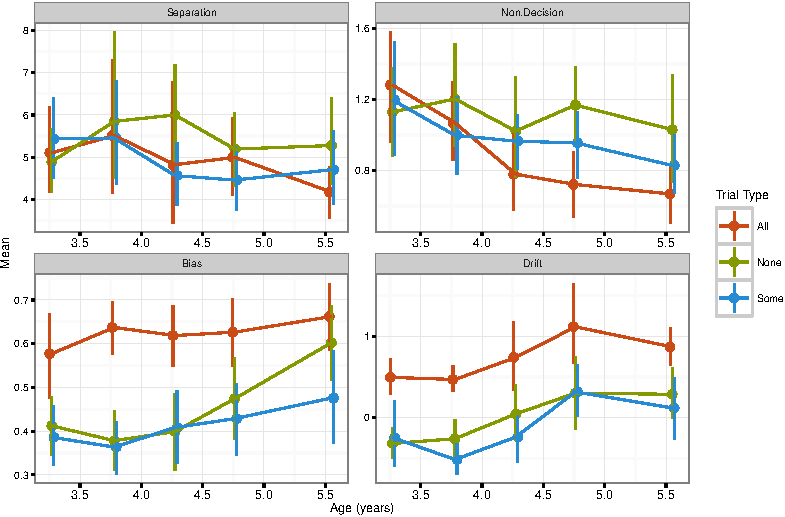
\includegraphics{figs/param_plot-1} 

}

\caption[Parameter estimates for drift diffusion model, split by age and trial type]{Parameter estimates for drift diffusion model, split by age and trial type. Error bars are 95 percent confidence intervals computed by nonparametric bootstrap.}\label{fig:param_plot}
\end{figure*}
\end{CodeChunk}

Using the DDM, we can explore in more depth the speed-accuracy tradeoff
we observed in both our statistical models. In our separation boundary
estimates, we saw that over development the boundary for a correct
response decreases, for all trial types, indicating that in general less
data needs to be accumulated before making a decision in this task. This
is also reflected in the bias estimates, which are very high for all age
groups on ``all'' trials, but increase over development for ``some'' and
``none'' trials. Interestingly, we found that non-decision decreases
markedly for ``all'' trials over development, but only slightly for
``some'' and ``none'' trials, while drift rates for all quantifiers
increase over development.

In this model, we find that younger children spend less time processing
a quantifier, and are also faster in making an incorrect decision with
the difficult quantifiers ``some'' and ``none''. Young children's high
drift rate and comparable nondecision estimates on ``all'' trials can be
attributed to their tendency to select the alternative for ``all'' on
the majority of trials. Later in development, however, we find that
older children seem to spend more time processing the quantifiers
``some'' and ``none'', and consequently are more likely to make a
correct response. Intriguigingly, we observe this trend even though
older children are have a greater bias and a lower separation boundary
with these quantifier types.

\section{General Discussion}\label{general-discussion}

Our primary question in this study centered on whether children who
succeed on a scalar implicature task (and also understand the
quantifiers involved) take more time to process. We adapted a previously
validated scalar implicature task (Horowitz \& Frank, 2015; Horowitz et
al., In prep.) for the iPad to explore whether children's success how
response latencies interacted with accuracy in this task.

In our analyses, we replicated previous results (Horowitz \& Frank,
2015; Horowitz et al., In prep.) in our finding that children were
overall less accurate when evaluting the quantifiers ``some'' and
``none'' in comparison to ``all,'' but that their performance increased
over development. We again found evidence of bimodal and correlated
performance on these two quantifier types, suggesting a common source of
difficulty.

In our extension of this paradigm, we collected reaction time data for
these quantifier types to investigate the relationship between reaction
time and accuracy. In our reaction time analyses, we found evidence of a
speed-accuracy tradeoff, as well as an interaction between reaction time
and age, with older children taking a slightly longer time to respond to
these trials, but ultimately being more accurate.

Using a Drift Diffusion Model, we explored reaction time and accuracy
patterns in more depth. Overall, the model predicted that children spend
more time processing these difficult pragmatic implicatures as they get
older, and are more likely to make a correct response as a result. Thus,
it appears that success in making a scalar implicature is not only the
result of being familiar with the quantifier scale, but also taking
additional time to process and integrate in a pragmatic framework in
order to make a response.

Our work contributes to the existing literature in utilizing a novel
method to collect accurate and detailed reaction time data on a scalar
implicature task. Response latencies are an important indicator of the
pragmatic challenges that children face in processing implicatures.
Additionally, our findings replicate previous work, providing evidence
for the appropriateness of this paradigm in targeting scalar
implicatures. Further, our larger sample size, increased number of
trials, and randomized design strengthen our analytical power, and allow
for more detailed inferences from the data.

(Final paragraph on quantifier knowledge, inhibitory control, scalar
implicatures, and how they relate more broadly to language).

\section{Acknowledgements}\label{acknowledgements}

Special thanks to Bing Nursery School, the San Jose Children's Discovery
Museum, Veronica Cristiano, Rachel Walker, and Tamara Mekler for their
help with data collection.

\section{References}\label{references}

\setlength{\parindent}{-0.1in} \setlength{\leftskip}{0.125in} \noindent

Barner, D., Chow, K., \& Yang, S. (2009). Finding one's meaning: A test
of the relation between quantifiers and integers in language
development. \emph{Cognitive Psychology}, \emph{58}(2), 195--219.

Grice, H. (1975). \emph{Logic and conversation} (pp. 41--58).

Guasti, M., Chierchia, G., Crain, S., Foppolo, F., Gualmini, A., \&
Meroni, L. (2005). Why children and adults sometimes (but not always)
compute implicatures. \emph{Language and Cognitive Processes},
\emph{20}(5), 667--696.

Horowitz, A., \& Frank, M. C. (2015). Sources of developmental change in
pragmatic inferences about scalar terms. In \emph{Proceedings of the
37th annual conference of the cognitive science society.}

Horowitz, A., Schneider, R. M., \& Frank, M. C. (In prep.). The trouble
with quantifiers: Children's difficulties with ``some'' and ``none''.

Huang, Y. T., \& Snedeker, J. (2009). Online interpretation of scalar
quantifiers: Insight into the semantics-pragmatics interface.
\emph{Cognitive Psychology}, \emph{58}(3), 376--415.

Katsos, N., \& Bishop, D. (2011). Pragmatic tolerance: Implications for
the acquisition of informativeness and implicature. \emph{Cognition},
\emph{120}(1), 67--81.

Milosavljevic, M., Malmaud, J., Huth, A., Koch, A., \& Rangel, A.
(2010). Drift diffusion model can account for accuracy and reaction time
of value-based choices under high and low time pressure. \emph{Judgment
and Decision Making}, \emph{5}(6), 437--449.

Noveck, I. (2001). When children are more logical than adults:
Experimental investigations of scalar implicature. \emph{Cognition},
\emph{78}(2), 165--188.

Papafragou, A., \& Musolino, J. (2003). Scalar implicatures: Experiments
at the semantics-pragmatics interface. \emph{Cognition}, \emph{86}(3),
253--282.

Papafragou, A., \& Tantalou, N. (2004). Children's computation of
implicatures. \emph{Language Acquisition}, \emph{12}, 71--82.

Ratcliff, R., \& Rouder, J. (1998). Modeling response times for
two-choice decisions. \emph{Psychologial Science}, \emph{9}(5),
347--356.

Zelazo, P. D. (2006). The dimensional change card sort (dCCS): A method
of assessing executive function in children. \emph{Nature Protocols},
\emph{1}, 297--301.

\end{document}
